\documentclass[letterpaper]{article}
%------------------------------------------------------------------------------------------
\title{Equations and Derivations for the Quaternion Python Module}
\author{Philippe Pinard}
\date{\today}
%------------------------------------------------------------------------------------------
\usepackage[letterpaper,top=2.5cm,bottom=2.5cm,right=2.5cm,left=2.5cm]{geometry}
\usepackage[english]{babel}
\usepackage[latin1]{inputenc}
%------------------------------------------------------------------------------------------
%\usepackage{fullpage}
\usepackage{graphicx}
\usepackage{subfigure}
\usepackage{multirow}
\usepackage{url}
\usepackage{amsmath}
\usepackage{amsfonts}
\usepackage{stmaryrd}
\usepackage{setspace}
\usepackage{sistyle}
\usepackage[nothing]{todo}
\usepackage[version=3]{mhchem}
\usepackage{fancyhdr}
\usepackage{paralist}
\usepackage{epic}
\usepackage{array}
%------------------------------------------------------------------------------------------
\usepackage[
	pdftitle={Equations and Derivations for the Pattern Simulations Python Module},
	pdfsubject={Programming notes},
	pdfkeywords ={pattern, lines, bands, plane spacing, Python, Derivations},
	pdfauthor={Philippe Pinard},
	colorlinks=true,
	linkcolor=blue,
	pdfborder=0 0 0,
	pdfhighlight=/I,
	pdfpagelabels]{hyperref}
%------------------------------------------------------------------------------------------

\DeclareMathAlphabet{\mathpzc}{OT1}{pzc}{m}{it}
\newcommand{\dev}{\ensuremath{\ \mathrm{d}}}
\renewcommand{\labelitemii}{$\diamond$}
\newcommand{\celsius}{^\circ C}
\renewcommand{\tablename}{Table}
\renewcommand{\figurename}{Figure}
\newcommand{\conj}[1]{#1^\ast}
\newcommand{\trans}[1]{#1^\mathrm{T}}
\newcommand{\vx}{\hat{x}}
\newcommand{\vy}{\hat{y}}
\newcommand{\vz}{\hat{z}}
\newcommand{\trace}[1]{\mathrm{Tr}(#1)}
\newcommand{\quaternion}[2]{\llbracket #1, #2 \rrbracket}
\newcommand{\quaternionL}[1]{\mathcal{#1}}
\newcommand{\norm}[1]{\left\|#1\right\|}
\newcommand{\im}{\mathit{i}}
\newcommand{\direction}[1]{\left[ #1 \right]}
\newcommand{\vecc}[3]{\left(#1,#2,#3\right)}
\newcommand{\var}[1]{\mathpzc{#1}}

\begin{document}
%------------------------------------------------------------------------------------------
	\pagestyle{fancy}
	\fancyhf{}
	\setlength{\headheight}{15pt}
	\setlength{\headsep}{10pt}
	\lhead{Equations and Derivations for the Pattern Simulations Python Module}
	\rhead{\today}
	\lfoot{\emph{Prepared by Philippe Pinard}}
	\rfoot{\thepage}
%------------------------------------------------------------------------------------------
	
	\section{Definitions and Notations}
	\subsection{Abbreviations}
		\begin{itemize}
			\item $\var{WD}$: Working Distance
			\item $\var{PC}$: Pattern center ($\var{PC}_x$: x coordinates of the pattern center)
			\item $\var{DD}$: Detector distance
			\item $hkl$: Plane coordinates
			\item $\vx$, $\vy$, $\vz$: Unit vectors of the reference axis system
		\end{itemize}
	\subsection{Reference Coordinates System}
		\begin{tabular}{p{0.3\textwidth}p{0.3\textwidth}p{0.3\textwidth}}
			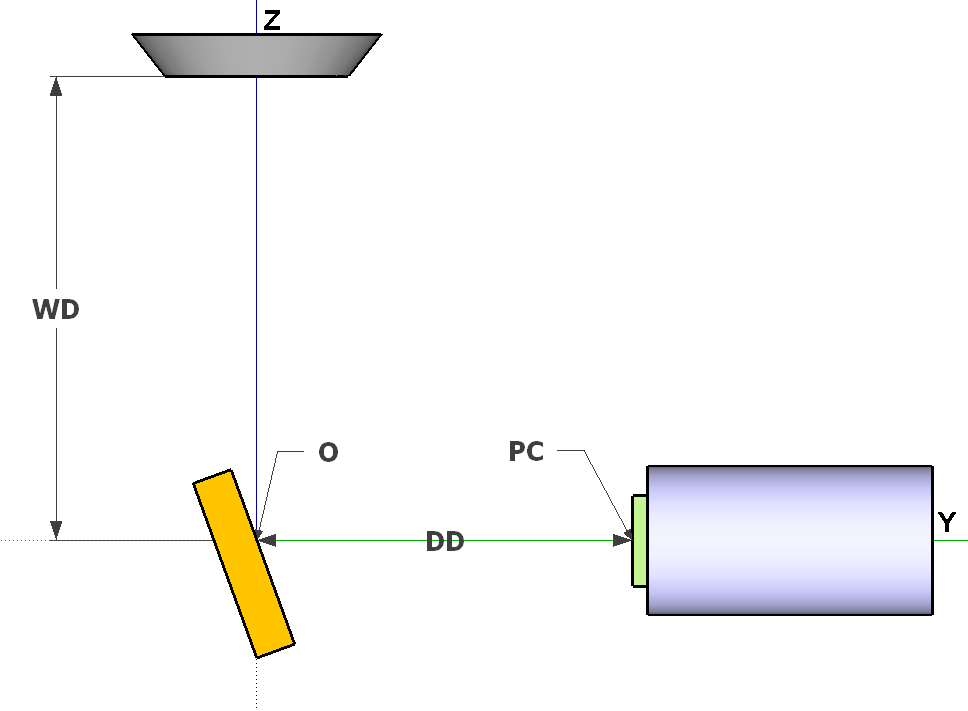
\includegraphics[width=0.3\textwidth]{figures/axis_system1} & 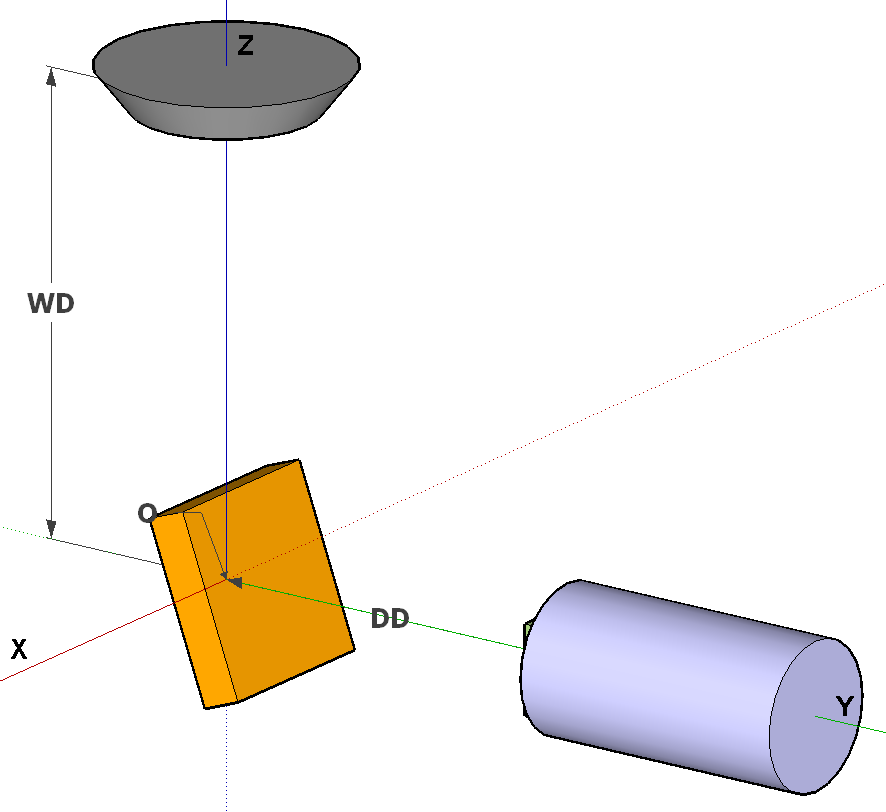
\includegraphics[width=0.3\textwidth]{figures/axis_system2} & 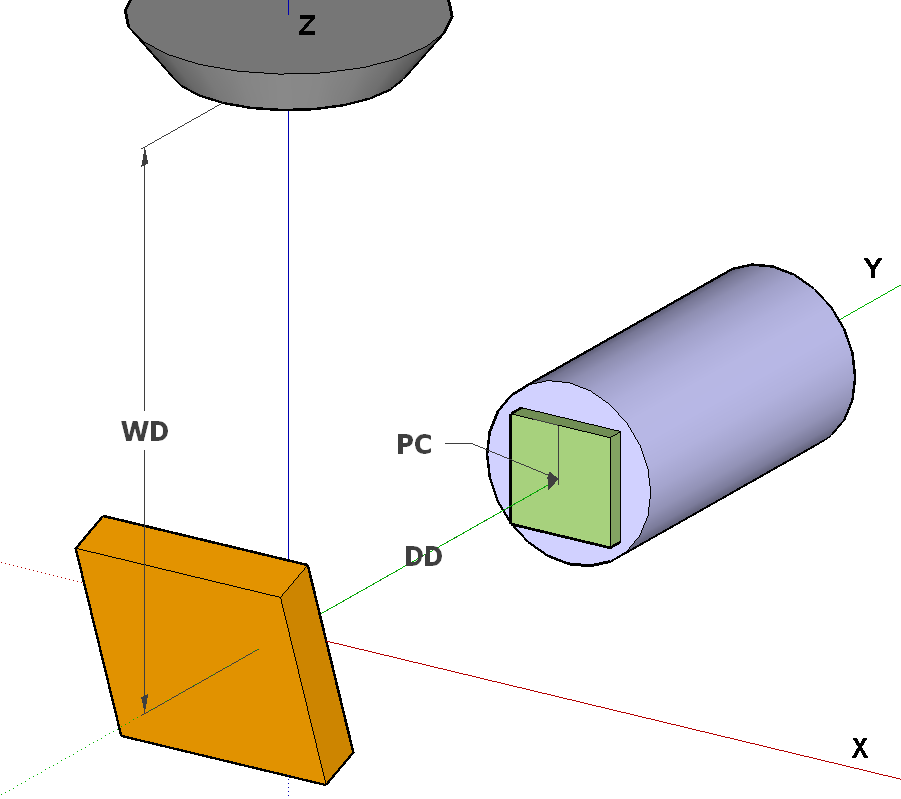
\includegraphics[width=0.3\textwidth]{figures/axis_system3} 
		\end{tabular}
		\begin{itemize}
			\item The origin of the reference coordinates system $\var{O}$ is taken as the point where the beam intersects the sample. To be more precise, the top left corner of the acquisition map.
			\item When the beam is scanned across the specimen, the $\var{PC}$ and $\var{DD}$ move as well. To simplify the calculations of the Kikuchi bands, the beam raster is taken into account before the calculations by converting the motion of the beam into a shift of the $\var{PC}$ and $\var{DD}$. Therefore, the point of incidence $\var{I}$ has always the coordinates $(0,0,0)$.
			\item The default position of the detector (i.e.\ without any correction of the detector orientation) is at $\var{DD}\vy$ of the sample.
			\item The default tilt axis is along the $\vx$ axis. Counter-clockwise rotation are taken as positive rotation.
			\item The coordinates of the $\var{PC}$ are always at $(\var{PC}_x, \var{DD}, \var{PC_z})$.
		\end{itemize}
	
	\subsection{Units}
	
	\section{Planes to Kikuchi bands}
	From planes representing a particular crystallographic orientation to their representations as Kikuchi bands on the detector, several steps are involved:
	\begin{enumerate}
		\item Reference coordinates system $\xrightarrow{\text{Specimen orientation}}$ Specimen coordinates system
		\item Specimen coordinates system $\xrightarrow{\text{Crystal orientation}}$ Crystal coordinates system
		\item Crystal coordinates system $\xrightarrow{\text{Tilt}}$ Tilted coordinates system
		\item Tilted coordinates system $\xrightarrow{\text{Detector orientation}}$ Detector corrected or Diffraction coordinates system
		\item Diffraction coordinates system $\rightarrow{\text{Diffraction}}$ Kikuchi bands
	\end{enumerate}
	
	\subsection{Specimen orientation}
	
	
	\subsection{Crystal orientation}
	
	\subsection{Tilt}
	
	
	\subsection{Detector orientation}
	
	\subsection{Diffraction}
	\subsubsection{Kikuchi Line}
	For a plane with a normal $\vec{n} = (n_x, n_y, n_z)$ and passing through the origin, the plane equation is:
	\begin{eqnarray}
		\vec{n} \cdot (x,y,z) & = & 0\\\nonumber
		n_xx + n_yy + n_zz & = & 0 
		\label{eq:plane}
	\end{eqnarray}
	
	Kikuchi lines (center of the Kikuchi bands) represent the intersection of diffracting planes with the detector.  
	This intersection of a plane with another plane is a line.
	To find the intersect of this plane, we can replace $(x,y,z)$ in Equation~\ref{eq:plane} by $(x, \var{DD}, z)$ since $y$ is fixed at $\var{DD}$ and write the line equation.
	\begin{eqnarray}
		n_x x + n_y \var{DD} + n_z z = 0 \\\nonumber
		z = -\frac{n_x}{n_z}x - \frac{n_y}{n_z}\var{DD}
		\label{eq:plane2}
	\end{eqnarray}
	
	Equation~\ref{eq:plane2} is incomplete, because it doesn't take into account the position of the pattern center, which might not be located at $(0,\var{DD},0)$. 
	For this correction, $x$ becomes $x-\var{PC}_x$ and $z$, $z-\var{PC}_z$.
	Rewriting the equation, we obtain:
	\begin{eqnarray}
		z = \left(-\frac{n_x}{n_z}\right)x + \left(\frac{n_x}{n_z}\var{PC}_x + - \frac{n_y}{n_z}\var{DD} + \var{PC}_z\right)
		\label{eq:plane3}
	\end{eqnarray}
	
	The slope is therefore $m=-\frac{n_x}{n_z}$ and the intercept $k=\frac{n_x}{n_z}\var{PC}_x + - \frac{n_y}{n_z}\var{DD} + \var{PC}_z$. We shall refer to the equation of Kikuchi line as Equation~\ref{eq:kikuchi_eq}.
	\begin{eqnarray}
		z = mx + k
		\label{eq:kikuchi_eq}
	\end{eqnarray}

	Equation~\ref{eq:plane3} is undetermined when $n_z = 0$. 
	This situations corresponds to a vertical line $x = \text{constant}$.
	\begin{eqnarray}
		n_x x + n_y \var{DD} + (0) z = 0 \\\nonumber
		x = -\frac{n_y}{n_x}\var{DD} + \var{PC}_x
		\label{eq:plane4}
	\end{eqnarray}
	
	Again there is a special case when $n_z = 0$ and $n_x = 0$, which corresponds to a plane parallel to the detector's plane. 
	There is no Kikuchi band for this case.
	
	\subsubsection{Kikuchi Bands}
	To determine the width of the Kikuchi Bands, we need to determine the scattering angle $\theta$ using the Bragg's Law. The wavelength $\lambda$ is determined from the electron's incident energy, and the plane spacing $d$ from the lattice parameters.
	\begin{eqnarray}
		\lambda = 2d\sin\theta
		\label{eq:bragg}
	\end{eqnarray}
	
	
	The scattering angle creates two Kikuchi cones (Figure~\ref{}). 
	It is the intersection of these cones with the detector that gives a width to the Kikuchi bands.
	The intersection of cones with a planes gives an hyperbola. 
	However, since the scattering angle is small for electron energies used in SEM, the hyperbola can be approximated as two lines. 
	So, to simplify the calculations, the cones are replaced by two planes separated by an angle $2\theta$.
	
	To convert the scattering angle $\theta$ to a distance on the detector $w$, we first find the smallest distance between the Kikuchi line and the origin. 
	This distance would correspond to half the distance between the two inflexion points of the hyperbola.
	This distance between a point and a line is given by the general Equation~\ref{eq:pointline}\ref{mathworld}, where $\vec{x}_0$ is the point, and $\vec{x}_1$ and $\vec{x}_2$ are two points on the line (Figure~\ref{fig:pointline}).
	\begin{eqnarray}
		d = \frac{\norm{(\vec{x}_2-\vec{x}_1) \times (\vec{x}_1-\vec{x}_0)}}{\norm{\vec{x}_2-\vec{x}_1}}
		\label{eq:pointline}
	\end{eqnarray}
	
	\begin{figure}
		\centering
		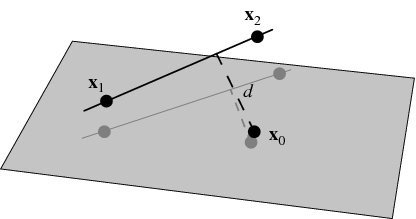
\includegraphics[width=0.3\textwidth]{figures/pointline}
		\caption{Distance between a point and a line}
		\label{fig:pointline}
	\end{figure}
	
	Using our \emph{Reference coordinates system}'s notation, $\vec{x}_0$ is the point of incidence $\var{I}$, and $\vec{x}_1$ and $\vec{x}_2$, as two points on the Kikuchi line, which we shall refer to as $\var{A}$ and $\var{B}$.  The selection of these two points requires to be discussed in more details since they are depend on the slope and intercept of the Kikuchi line (Figure~\ref{fig:cases}).
	\begin{enumerate}
		\item Vertical line ($x=\text{constant}$)
			\begin{itemize}
				\item $\var{A} = \left(k, \var{DD}, 0\right)$
				\item $\var{B} = \left(k, \var{DD}, 0.1\right)$
			\end{itemize}
		\item Horizontal line ($z=k$)
			\begin{itemize}
				\item $\var{A} = \left(0, \var{DD}, k\right)$
				\item $\var{B} = \left(0.1, \var{DD}, k\right)$
			\end{itemize}
		\item Oblique line when $k=0$ ($z=mx$)
			\begin{itemize}
				\item $\var{A} = \left(0, \var{DD}, 0\right)$ (case when $x=0$)
				\item $\var{B} = \left(\frac{1}{m}, \var{DD}, 1\right)$ (case when $z=1$)
			\end{itemize}
		\item Oblique line ($z=mx+k$)
			\begin{itemize}
				\item $\var{A} = \left(0, \var{DD}, k\right)$ (case when $x=0$)
				\item $\var{B} = \left(\frac{-k}{m}, \var{DD}, 0\right)$ (case when $z=0$)
			\end{itemize}
	\end{enumerate}
	
	\begin{figure}
		\centering
		
		\begin{tabular}{cc}
		Vertical line ($x=\text{constant}$) & Horizontal line ($z=k$) \\
		\begin{picture}(150,100)
			\put(10,10){\line(1,0){130}}
			\put(10,10){\line(0,1){80}}
			\put(10,90){\line(1,0){130}}
			\put(140,10){\line(0,1){80}}
			
			\put(30,20){\vector(-1,0){10}}
			\put(30,20){\vector(0,1){10}}
			\put(18,22){$x$}
			\put(33,27){$z$}
			
			\thicklines
			\put(60,10){\line(0,1){80}}
			\put(60, 30){\circle*{4}}
			\put(65, 30){$\var{A}\;(k,0)$}
			\put(60, 70){\circle*{4}}
			\put(65, 70){$\var{B}\;(k,0.1)$}
		\end{picture}
		&
		\begin{picture}(150,100)
			\put(10,10){\line(1,0){130}}
			\put(10,10){\line(0,1){80}}
			\put(10,90){\line(1,0){130}}
			\put(140,10){\line(0,1){80}}
			
			\put(30,20){\vector(-1,0){10}}
			\put(30,20){\vector(0,1){10}}
			\put(18,22){$x$}
			\put(33,27){$z$}
			
			\thicklines
			\put(10,60){\line(1,0){130}}
			\put(30, 60){\circle*{4}}
			\put(30, 65){$\var{A}\;(0,k)$}
			\put(100, 60){\circle*{4}}
			\put(100, 65){$\var{B}\;(0.1,k)$}
		\end{picture} \\
		
		Oblique line when $k=0$ ($z=mx$) & Oblique line ($z=mx+k$) \\
		\begin{picture}(150,100)
			\put(10,10){\line(1,0){130}}
			\put(10,10){\line(0,1){80}}
			\put(10,90){\line(1,0){130}}
			\put(140,10){\line(0,1){80}}
			
			\put(30,70){\vector(-1,0){10}}
			\put(30,70){\vector(0,1){10}}
			\put(18,62){$x$}
			\put(33,77){$z$}
			
			\thicklines
			\put(10,10){\line(3,2){120}}
			\put(30, 23){\circle*{4}}
			\put(35, 18){$\var{A}\;(0,0)$}
			\put(100, 70){\circle*{4}}
			\put(105, 65){$\var{B}\;(\frac{1}{m},1)$}
		\end{picture}
		&
		\begin{picture}(150,100)
			\put(10,10){\line(1,0){130}}
			\put(10,10){\line(0,1){80}}
			\put(10,90){\line(1,0){130}}
			\put(140,10){\line(0,1){80}}
			
			\put(30,70){\vector(-1,0){10}}
			\put(30,70){\vector(0,1){10}}
			\put(18,62){$x$}
			\put(33,77){$z$}
			
			\thicklines
			\put(10,40){\line(5,2){125}}
			\put(30, 48){\circle*{4}}
			\put(35, 43){$\var{A}\;(0,k)$}
			\put(100, 76){\circle*{4}}
			\put(105, 71){$\var{B}\;(-\frac{k}{m},1)$}
		\end{picture}
		\end{tabular}
		
		\label{fig:cases}
		\caption{Four different cases of Kikuchi lines}
	\end{figure}
	
	
	Let define the normal of the plane form by points $\var{I}$, $\var{A}$ and $\var{B}$ as $\vec{N}$ as seen in Figure~\ref{fig:widthangle1}. Note that in Figure~\ref{fig:widthangle1}, the origin of the axes is located at $(0,\var{DD},0)$ to illustrate better the positions relative to the detector screen. Equation~\ref{eq:pointline} can be re-written using the new defined points.
	\begin{eqnarray}
		d = \frac{\norm{\vec{N}}}{\norm{\overrightarrow{\var{AB}}}}
		\label{eq:pointline2}
	\end{eqnarray}
	
	\begin{figure}
		\centering
		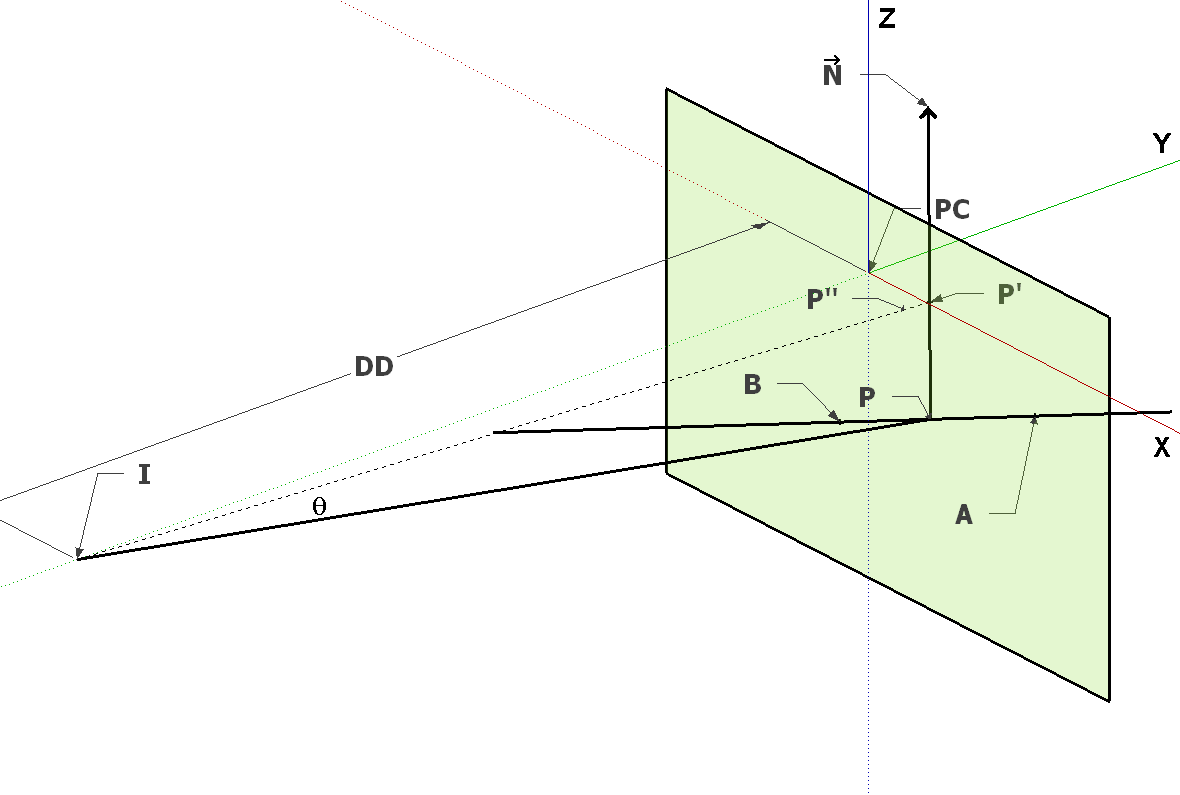
\includegraphics[width=0.8\textwidth]{figures/widthangle1}
		\caption{Schematics of points and vectors to find the distance between $\var{I}$ and the Kikuchi line $\var{AB}$}
		\label{fig:widthangle1}
	\end{figure}
	
	From Figure~\ref{fig:widthangle}, we have the following orthogonality relations:
	\begin{eqnarray}
		\overrightarrow{\var{IP}} \cdot \vec{N} & = & 0 \; (\angle\var{IPP^\prime} = \pi/2)\\
		\overrightarrow{\var{AB}} \cdot \vec{N} & = & 0 \; (\angle\var{APP^\prime} = \angle\var{BPP^\prime} = \pi/2)\\
		\overrightarrow{\var{IP}} \cdot \overrightarrow{\var{AB}} & = & 0 \; (\angle\var{IPA} = \angle\var{IPB} = \pi/2)
		\label{eq:orthogonality}
	\end{eqnarray}
	
	Excepted when the Kikuchi line passes through the pattern center, the normal $\vec{N}$ is not parallel to the detector screen, forming an angle $\alpha$ with the latter. To solve for the width of the band $\norm{\overrightarrow{\var{PP}^{\prime\prime}}}$ we introduce the vector $\vec{S}$, which is defined as a vector parallel to the detector screen and perpendicular to $\overrightarrow{\var{AB}}$. The coordinates of $\vec{s}$ are therefore $(N_x, 0, N_z)$. Figure~\ref{fig:widthangle2}, which is a projection in the $x$-direction of Figure~\ref{fig:widthangle1}, illustrates the definition of $\vec{S}$ and $\alpha$.
	
	\begin{figure}
		\centering
		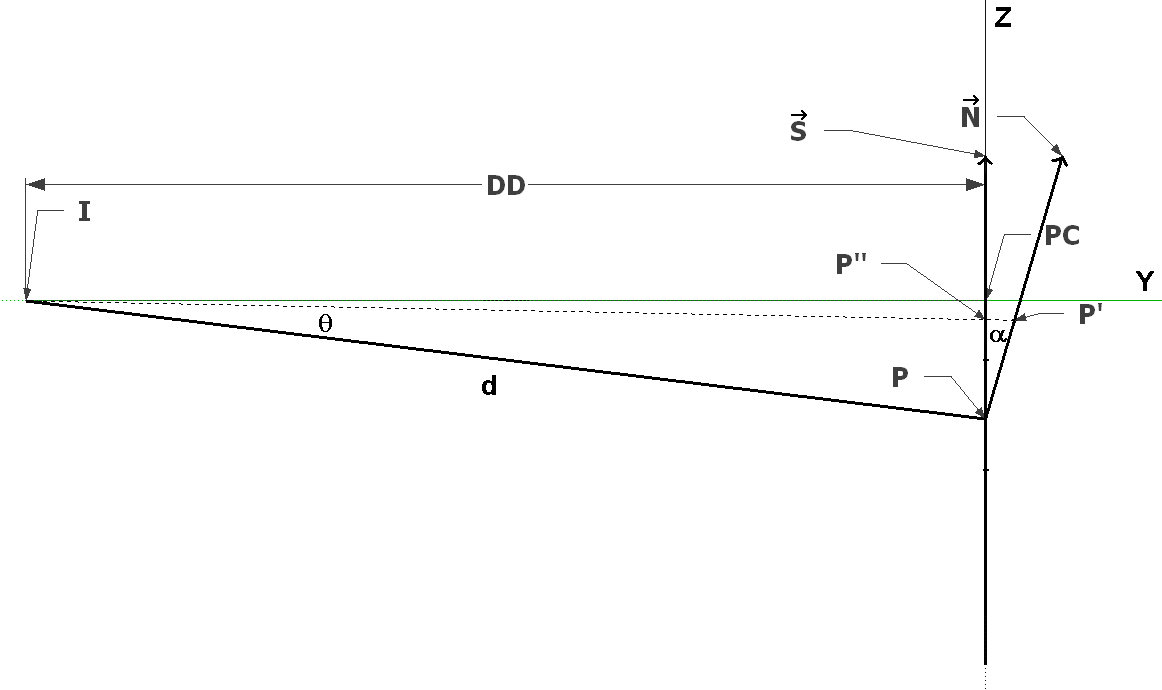
\includegraphics[width=0.8\textwidth]{figures/widthangle2}
		\caption{Schematics of points, vectors and angles to find the distance between $\var{P}$ and $\var{P}^{\prime\prime}$ above the Kikuchi line $\var{AB}$}
		\label{fig:widthangle2}
	\end{figure}
	
	The angle $\alpha$ can be calculated using the dot product of vectors $\vec{S}$ and $\vec{N}$. 
	\begin{eqnarray}
		\alpha = \arccos{\frac{\vec{S}\cdot\vec{N}}{\norm{\vec{S}}\norm{\vec{N}}}}
		\label{eq:alpha}
	\end{eqnarray}
	
	The vectors $\vec{S}$ and $\vec{N}$ forms a scalene triangle $\triangle\var{PP^\prime P^{\prime\prime}}$. 
	Knowing that the $\angle\var{PP^\prime P^{\prime\prime}} = \frac{\pi}{2}-\theta$ and $\angle\var{P^\prime PP^{\prime\prime}} = \alpha$, the $\angle\var{PP^{\prime\prime}P^\prime}$ is equal to $\frac{\pi}{2} + \theta - \alpha$. 
	Using the Sin's Law, the following relation can be established:
	\begin{eqnarray}
		\frac{\sin{\left(\frac{\pi}{2} + \theta - \alpha\right)}}{\norm{\overrightarrow{\var{PP^\prime}}}} = \frac{\sin{\left(\frac{\pi}{2} - \theta\right)}}{\norm{\overrightarrow{\var{PP^{\prime\prime}}}}}
		\label{eq:sinlaw}
	\end{eqnarray}
	
	Knowing that $\norm{\overrightarrow{\var{PP^\prime}}} = d\tan\theta$ and solving for $\norm{\overrightarrow{\var{PP^{\prime\prime}}}}$, we obtain
	\begin{eqnarray}
		\norm{\overrightarrow{\var{PP^{\prime\prime}}}} = d\tan\theta \frac{\sin{\left(\frac{\pi}{2} - \theta\right)}}{\sin{\left(\frac{\pi}{2} + \theta - \alpha\right)}} = d\tan\theta \frac{\cos{\theta}}{\cos{\left(\alpha - \theta\right)}} = d \frac{\sin{\theta}}{\cos{\left(\alpha - \theta\right)}}
		\label{eq:width1}
	\end{eqnarray}
	
	The Kikuchi bands also extends below the Kikuchi line. To calculate this distance we can use the same relationships as for the one above (Figure~\ref{fig:widthangle3}. 
	We obtain:
	\begin{eqnarray}
		\norm{\overrightarrow{\var{PQ^{\prime\prime}}}} = d \frac{\sin{\theta}}{\cos{\left(\alpha + \theta\right)}}
		\label{eq:width2}
	\end{eqnarray}
	
	\begin{figure}
		\centering
		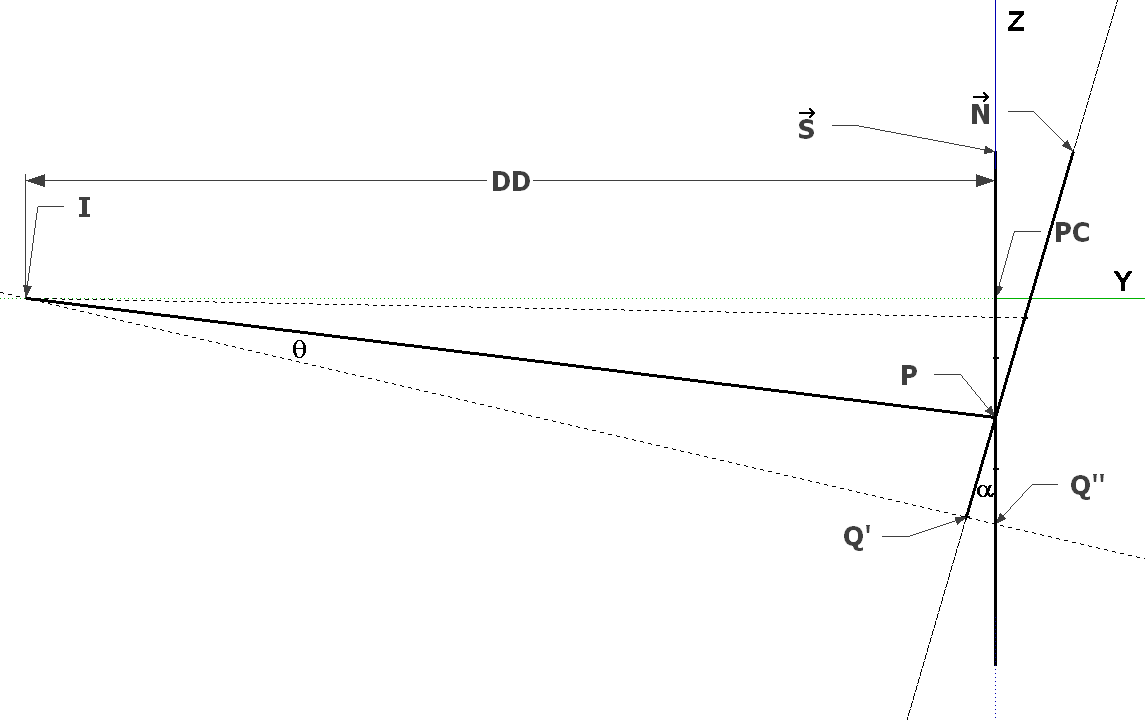
\includegraphics[width=0.8\textwidth]{figures/widthangle3}
		\caption{Schematics of points, vectors and angles to find the distance between $\var{P}$ and $\var{P}^{\prime\prime}$ below the Kikuchi line $\var{AB}$}
		\label{fig:widthangle3}
	\end{figure}
	
	Equation~\ref{eq:width1} and \ref{eq:width2}, as well as Figure~\ref{fig:widthangle3} show that the half-widths of a Kikuchi band are not equal.
	When drawing filled Kikuchi bands, we will approximate that the half-widths are the same and equal to half the total width. 
	This approximate introduces an error less than 10\% on the center of the band.
	\begin{eqnarray}
		w = d \sin{\theta} \left[\sec{\left(\alpha - \theta\right)} + \sec{\left(\alpha + \theta\right)}\right]
		\label{eq:totalwidth}
	\end{eqnarray}
	
	However, when drawing the edges of the bands, the difference between the half-widths will be taken into account.
	For the equations for the lines representing the edges, they will have the same slope as the Kikuchi line, $m$, but a different intercept, $k$.
	As defined above, the half-widths found are perpendicular to the Kikuchi line. 
	Therefore, to determine the intercept of the edges, we need to find the variation in $z$ ($h$) related to the half-widths.
	As seen in Figure~\ref{fig:widthangle4}, 
	\begin{eqnarray}
		h = \norm{\overrightarrow{\var{PP^{\prime\prime}}}} \cos\beta\\
		h^\prime = \norm{\overrightarrow{\var{PQ^{\prime\prime}}}} \cos\beta
		\label{eq:height1}
	\end{eqnarray}
	where $\beta$ is the angle with respect to the $x$-axis of the Kikuchi line $\var{AB}$.
	The angle $\beta$ can be calculated using the slope of the Kikuchi line.
	\begin{eqnarray}
		\beta = \arctan{m}
		\label{eq:beta}
	\end{eqnarray}
	
	\begin{figure}
		\centering
		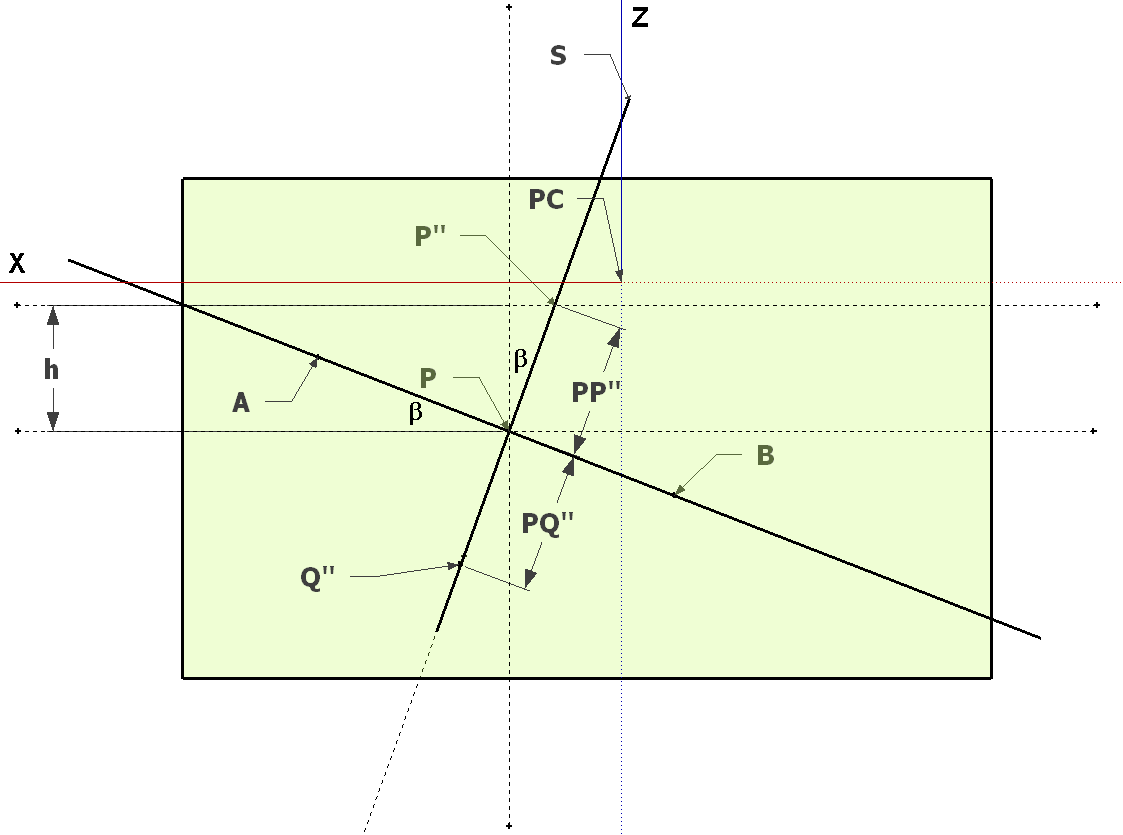
\includegraphics[width=0.8\textwidth]{figures/widthangle4}
		\caption{Schematics of points, vectors and angles to find the intercepts of the Kikuchi band' edges}
		\label{fig:widthangle4}
	\end{figure}
	
	The equations of the two edges are:
	\begin{itemize}
		\item $z = mx + k + h$
		\item $z = mx + k - h^\prime$
	\end{itemize}
	
	\subsection{Bands Intensity}
	
	
\end{document}

		
%	\begin{picture}(300,200)
%		%Axis 3D
%%		\put(10,10){\vector(0,1){20}}
%%		\put(10,10){\vector(1,0){20}}
%%		\put(10,10){\vector(-1,-1){10}}
%%		\put(13,25){\small{$z$}}
%%		\put(25,3){\small{$y$}}
%%		\put(-2,5){\small{$x$}}
%		\includegraphics[width=0.5\textwidth]{figures/axis_system}
%		%Axis 2D
%		\put(10,10){\vector(0,1){20}}
%		\put(10,10){\vector(1,0){20}}
%		\put(6,7.5){$\varotimes$}
%		\put(13,25){\small{$z$}}
%		\put(25,3){\small{$y$}}
%		\put(2,2){\small{$x$}}
%		
%		
%	\end{picture}
%	